\section*{Introduction}

How biology produces robust pattern in space and time is still largely an open question.
In 1952, Alan Turing proposed a mechanism referred to as Turing patterns or diffusion-driven instabilities, which explains how a homogeneous tissue results in self-organized spatial repetitive patterns of the network’s molecules.
However, this proposed mechanism is far from real biological complexity, and suffers from fine tuning, meaning only a small subset of constrained parameters can generate these spatial patterns.
Additionally, the diffusion-driven instability is based on linear stability analysis theory meaning natural relevant phenomena such as multistability, growth, exotic boundary conditions and non-linearities are often not addressed.
A way forward to understanding the relationship between theoretical Turing patterns and real biological patterns is to engineer these reaction-diffusion networks in biofilms using synthetic biology.
This would allow us to better understand the role of Turing patterns in biological pattern formation, as well as to engineer synthetic patterns for industrial applications.
This approach was implemented in~\cite{Oliver2023} where a Turing gene circuit was introduced in growing \textit{E.coli} colonies producing periodic spatial patterns (See Fig.~\ref{fig1}A).

Such a system has non-linearities, multistability, growth and absorbing boundary conditions which are not easily captured with linear stability analysis.
Several studies have explored how these phenomena affect Turing pattern formation including non-linearities~\parencite{ermentrout1991stripes}, multistability~\parencite{Krause2023}, boundaries~\parencite{Arcuri1986,Maini1993, Maini1997,Krause2020, Krause2021, Woolley2022} and growth~\parencite{gaffney2010, Klika2017, Krause2019}.
However, these studies are often based on idealised domains, certain types of popular BCs, and artificial growth assumptions.
Additionally, often they do not provide statistics of how Turing patterns become more or less robust to the fine-tuning problem when introducing these phenomena by conducting high-throughput parameter scans.
Therefore, a high-throughout numerical study is needed to understand how all these natural phenomena affect Turing pattern formation, in particular in a synthetic system such as the one in~\cite{Oliver2023}.

In this paper, we combine linear stability analysis and numerics, to study a simple turing network with non-linearities and multistability.
Our analysis goes beyond classical Turing patterns as we look at other types of instabilities such as Hopf and Turing-Hopf and how these can generate periodic stationary or non-stationary patterns.
We find that switching of steady states in multistable system can generate unexpected outcomes not predicted by linear stability analysis.
Additionally, growth and realistic boundary conditions are added to understand how patterning occurs in microbial colonies with synthetic Turing gene circuits (See Fig.~\ref{fig1}B-C).
We find that different boundaries and growing regimes can break or form patterns, therefore adding or removing robustness to pattern formation.
Studying how all these biological phenomena affect patterning is extremely important not only in the context of engineering patterns in synthetic biology systems, but also to understand how robust patterns occur developmental biology where large networks exhibit non-linearities and multistability and where tissues are growing and in contact with an external environments.


% Place figure captions after the first paragraph in which they are cited.
\begin{figure}[H]
    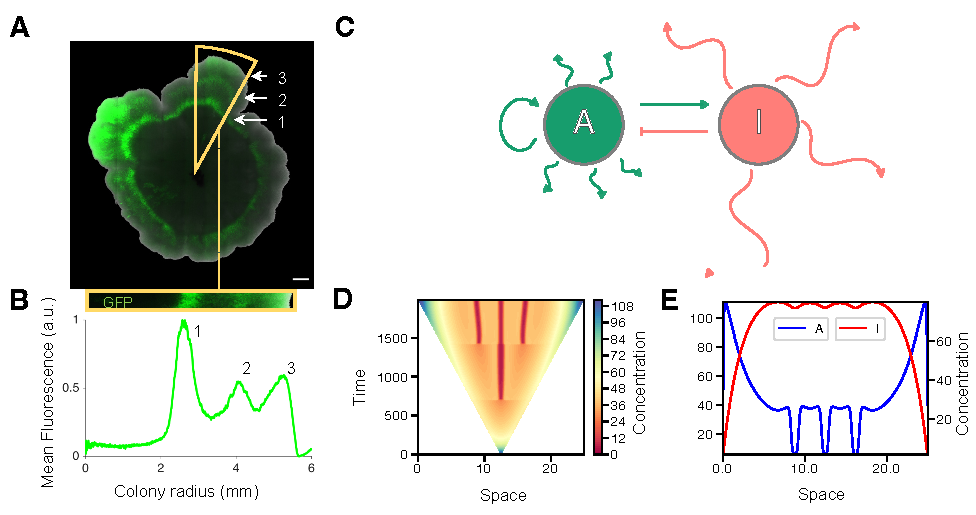
\includegraphics[width=1\textwidth]{figures/biological_example}

    \caption{{\bf Experiments and modelling of synthetic patterns.}
        \textbf{(A)} Xh snapshot of bacterial colony with 6-node Turing gene circuit produces periodic spatial patterns in 2D. Cross section of the colony to observe the periodic pattern in 1D is shown in white. \textbf{(B)} 1D simulation final snapshot of growing field with absorbing boundary conditions generates periodic pattern. Y axis is concentration (nM) of U (left, blue) and V (right, red) while X axis is space (mm). \textbf{(C)} Simulation shown in B, plotted as timeseries of molecule U. Y axis is time (h), X axis is space (mm) and concentration is shown by color with blue being high concentration and red being low concentration. }
    %TODO figure caption
    \label{fig1}
\end{figure}
 